% UPLOAD FINAL PDF TO:
%
%    https://indico.cern.ch/event/637013/contributions/2739332/
%
% TIME
%
%    Thu 19 Oct 2017, 12h15
%    20 mins + 5 mins for questions
%
% TITLE
%
%    The Outlook for Archival Storage at CERN
%
% ABSTRACT
%
%    The CERN Physics Archive is projected to reach 1 Exabyte during LHC Run 3. As the custodial copy of
%    the data archive is stored on magnetic tape, it is very important to CERN to predict the future of
%    tape as a storage medium.
%
%    This talk will give an overview of recent developments in tape storage, and a look forward to how
%    the archival storage market may develop over the next decade. The presentation will include a status
%    update on the new CERN Tape Archive software.

\documentclass{beamer}
\usetheme{Frankfurt}
\usecolortheme{beaver} 

% Remove navigation symbols
\setbeamertemplate{navigation symbols}{}

% Change bullet points
\setbeamertemplate{itemize items}[square]


% Add page number to top bar

\newcounter{num}
\newcounter{totalnum}

\def\pagenumbers#1#2{\expandafter\ifnum#1>#2\relax\else{\large#1}/#2\fi}

\makeatletter
\defbeamertemplate*{headline}{my smoothbars theme}
{%
  \setcounter{num}{\insertframenumber}%
  \addtocounter{num}{-1}%
  \setcounter{totalnum}{\inserttotalframenumber}%
  \addtocounter{totalnum}{-5}%
  \pgfuseshading{beamer@barshade}%
  \ifbeamer@sb@subsection%
    \vskip-9.75ex%
  \else%
    \vskip-7ex%
  \fi%
  \begin{beamercolorbox}[ignorebg,ht=2.25ex,dp=3.75ex]{section in head/foot}
    \insertnavigation{.9\paperwidth}\hfill\raisebox{-2ex}{\pagenumbers{\thenum}{\thetotalnum}}\hspace{.5em}
  \end{beamercolorbox}%
  \ifbeamer@sb@subsection%
    \begin{beamercolorbox}[ignorebg,ht=2.125ex,dp=1.125ex,%
      leftskip=.3cm,rightskip=.3cm plus1fil]{subsection in head/foot}
      \usebeamerfont{subsection in head/foot}\insertsubsectionhead
    \end{beamercolorbox}%
  \fi%
}%
\makeatother

% List of what areas setbeamercolor can change
% 
% abstract
% abstract title
% alerted text
% author
% author in head/foot
% author in sidebar
% background
% background canvas
% bibliography entry author
% bibliography entry location
% bibliography entry note
% bibliography entry title
% bibliography item
% block body
% block body alerted
% block body example
% block title
% block title alerted
% block title example
% button
% button border
% caption
% caption name
% date
% date in head/foot
% date in sidebar
% description item
% enumerate item
% enumerate subitem
% enumerate subsubitem
% example text
% fine separation line
% footline
% framesubtitle
% frametitle
% frametitle right
% headline
% institute
% institute in head/foot
% institute in sidebar
% item
% item projected
% itemize item
% itemize subitem
% itemize subsubitem
% itemize/enumerate body
% itemize/enumerate subbody
% itemize/enumerate subsubbody
% local structure
% logo
% lower separation line foot
% lower separation line head
% math text
% math text displayed
% math text inlined
% middle separation line foot
% middle separation line head
% mini frame
% navigation symbols
% navigation symbols dimmed
% normal text
% normal text in math text
% normal text in math text
% page number in head/foot
% palette primary
% palette quaternary
% palette secondary
% palette sidebar primary
% palette sidebar quaternary
% palette sidebar secondary
% palette sidebar tertiary
% palette tertiary
% part name
% part title
% qed symbol
% quotation
% quote
% section in head/foot
% section in sidebar
% section in sidebar shaded
% section in toc
% section in toc shaded
% section name
% section number projected
% section title
% separation line
% sidebar
% sidebar left
% sidebar right
% structure
% subitem
% subitem projected
% subsection in head/foot
% subsection in sidebar
% subsection in sidebar shaded
% subsection in toc
% subsection in toc shaded
% subsection name
% subsection number projected
% subsection title
% subsubitem
% subsubitem projected
% subsubsection in head/foot
% subsubsection in sidebar
% subsubsection in sidebar shaded
% subsubsection in toc
% subsubsection in toc shaded
% subsubsection number projected
% subtitle
% title
% title in head/foot
% title in sidebar
% titlegraphic
% titlelike
% upper separation line foot
% upper separation line head
% verse

% CERN blue is Pantone 286 = RGB 56 97 170, defined as cern@blue below

\definecolor{cern@ltblue}{rgb}{0.415686,0.611765,0.964706} % RGB 106 156 246
\definecolor{cern@blue}  {rgb}{0.219608,0.380392,0.666667} % RGB  56  97 170
\definecolor{cern@dkblue}{rgb}{0.082353,0.184314,0.364706} % RGB  21  47  93

% Complimentary colours

\definecolor{cern@ltcomp}{rgb}{0.666667,0.525490,0.219608} % RGB 170 134  56
\definecolor{cern@dkcomp}{rgb}{0.364706,0.266667,0.047059} % RGB  93  68  12

\setbeamercolor{title}                   {bg=cern@blue,fg=white}
\setbeamercolor{frametitle}              {bg=cern@blue,fg=white}
\setbeamercolor{section in head/foot}    {bg=cern@ltblue,fg=white}
\setbeamercolor{structure}               {fg=cern@dkcomp}
\setbeamercolor{bibliography entry title}{fg=cern@ltblue}

%
% Get packages that we need
%

% Change fonts to Avenir
% Note: need to compile with xelatex to use this package
\usepackage{fontspec}
\setsansfont{AvenirLTStd-Book}

%\usepackage[showboxes,overlay,absolute]{textpos}
\usepackage[overlay,absolute]{textpos}
\setlength{\TPHorizModule}{.01\paperwidth} % Horizontal units are percent of paper width
\setlength{\TPVertModule}{.01\paperwidth}  % Make vertical units equal to horizontal units
\textblockorigin{.5\paperwidth}{4.25ex}

% Headings within slides
\usepackage{xcolor}

\usepackage{tabularx}
\usepackage{enumitem}
\setitemize{label=\usebeamerfont*{itemize item}%
  \usebeamercolor[fg]{itemize item}
  \usebeamertemplate{itemize item}}

\newcommand\colhead[1]{\fontspec{Humanst521 BT}\textcolor{cern@dkblue}{\small\textbf{#1}}}

\newcommand\boxhead[1]{%
  \par\begin{center}
  \fontspec{Humanst521 BT}\textcolor{cern@dkblue}{\textbf{#1}}
  \end{center}\par}

% Shortcuts to handle 1st, 2nd, 3rd, 4th
\newcommand{\superscript}[1]{\ensuremath{^{\textrm{#1}}}}
\newcommand{\subscript}[1]{\ensuremath{_{\textrm{#1}}}}
\newcommand{\st}[0]{\superscript{st} }
\newcommand{\nd}[0]{\superscript{nd} }
\newcommand{\rd}[0]{\superscript{rd} }
\renewcommand{\th}[0]{\superscript{th} }

%
% Citation aliasing
%

\let\oldbibitem=\bibitem
\renewcommand{\bibitem}[2][]{\label{mybib#2}\oldbibitem[#1]{#2}}
%\newcommand\citealias[2]{\hyperlink{bib#1}{#2}\phantom{\cite{#1}}}
%\newcommand\citealias[2]{\cite[#2]{#1}}
\newcommand\citealias[2]{\hyperlink{mybib#1}{#2}\phantom{\cite{#1}}}


\begin{document}

%%
%% Title Page
%%

{
\setbeamertemplate{headline}{}
\begin{frame}
\begin{center}
\vspace{-4ex}

\includegraphics[width=0.25\textwidth]{images/CERN_logo}\\[2ex]
\color{cern@dkblue}
{\Huge\fontspec{Humanst521 BT} The Outlook for Archival\\[0.5ex]
Storage at CERN}\\[2ex]
{\Large Michael Davis and Germ\'{a}n Cancio}\\[2ex]
\color{cern@dkcomp}
Storage Group~\textbullet~IT Department~\textbullet~CERN\\[1ex]
19 October 2017
\end{center}
\end{frame}
}

\color{cern@dkblue}

%%
%% SECTION 1
%%

\section{Introduction}
\subsection{Introduction}

\begin{frame}{Overview}{}
{\Large
\begin{itemize}
   \item Roadmap for Tape
   \item Roadmap for Disk
   \item Alternatives to Tape
   \item Archival at CERN 
\end{itemize}
}
\end{frame}



\section{Tape Roadmap}
\subsection{Tape Roadmap}

\begin{frame}{Tape Market}{}
{\Large Market dominated by LTO consortium ($\approx$95\%)}

\begin{itemize}
   \item \textbf{Drives:} IBM, HP, Quantum. Oracle resells LTO drives from IBM, HP.
   \item \textbf{Media:} Fujifilm, Sony. TDK exited the tape media market in 2014.
\end{itemize}

{\Large Enterprise Tape: IBM, Oracle ($\approx$4\%)}

\begin{itemize}
   \item \textbf{Latest IBM Drive:} TS1155 (introduced May 2017; 15 Tb, 350 Mb/s)
   \item \textbf{Latest Oracle Drive:} T10KD (introduced September 2013; 8TB, 250 Mb/s)
\end{itemize}

{\Large Large-scale libraries ($\geq$ 10K slots)}

\begin{itemize}
   \item Oracle, IBM, Spectra Logic, now also Quantum
\end{itemize}
\end{frame}



\begin{frame}{Tape Drive Head Technology}{}
{\Large From Giant MagnetoResistive (GMR)\\
\hfill to Tunnel MagnetoResistive (TMR)}
\bigskip
\begin{itemize}
   \item TMR is 6$\times$ more sensitive than GMR
   \item HDDs have been using TMR since 2005
   \item GMR has reached its density limits for tape
   \item IBM TS1155 uses TMR
   \item LTO-8 will use it
\end{itemize}
\end{frame}



% IBM demos use sputtered media and TMR reader
\begin{frame}{Tape Track Density}{Source: \citealias{ibm_tape_roadmap}{IBM DACH (2015)}}
\begin{textblock}{90.0}[0.5,1](0,65) % {block width} (coords)
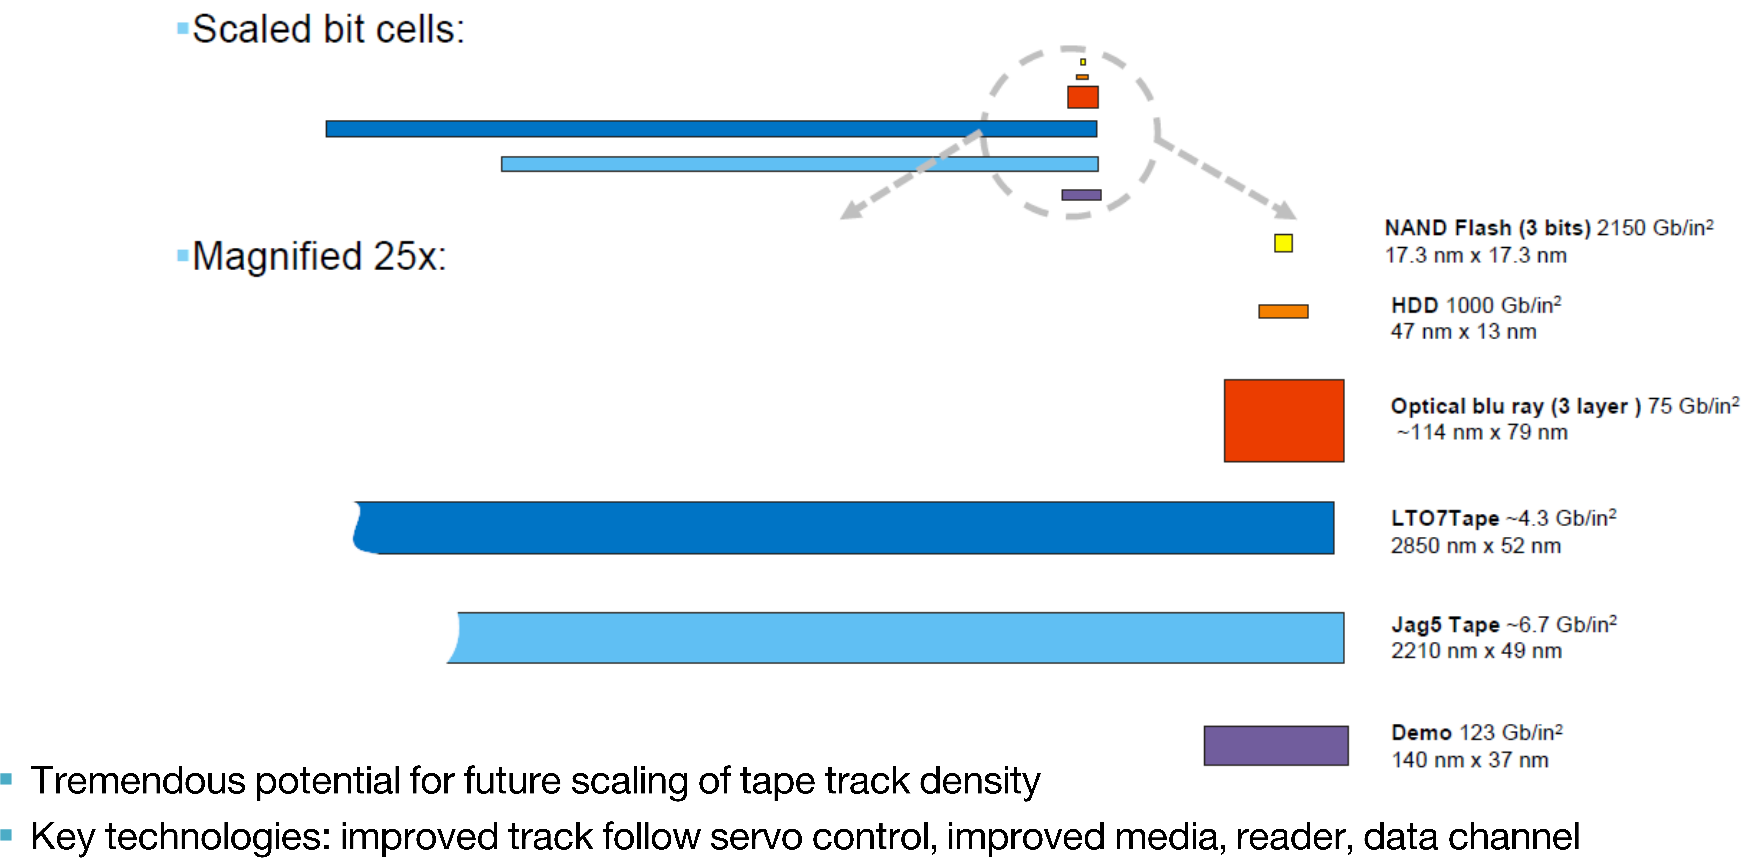
\includegraphics[width=\textwidth]{images/StorageBitCellsExtendibility.png}
\end{textblock}
%\begin{itemize}
   %\item Tremendous potential for future scaling of tape track density
   %\item Key technologies: improved track follow servo control, improved media, reader, data channel
%\end{itemize}
\end{frame}



\begin{frame}{Aereal Density Trends}{Source: \citealias{insic_roadmap}{INSIC (2016)}}
\begin{textblock}{90.0}[0.52,1](0,68) % {block width} (coords)
\includegraphics<1>[width=0.95\textwidth]{images/ArealDensity0.png}
\includegraphics<2>[width=0.95\textwidth]{images/ArealDensity1.png}
\includegraphics<3>[width=0.95\textwidth]{images/ArealDensity2.png}
\includegraphics<4>[width=0.95\textwidth]{images/ArealDensity3.png}
\end{textblock}
\end{frame}



\begin{frame}{LTO/IBM Enterprise Tape Roadmap}{Source: \citealias{ibm_tape_roadmap}{IBM DACH (2015)}}
\begin{textblock}{100.0}[0.5,1](0,70) % {block width} (coords)
\includegraphics<1>[width=\textwidth]{images/TapeDriveHistoryAndRoadMap0.png}
\includegraphics<2>[width=\textwidth]{images/TapeDriveHistoryAndRoadMap1.png}
\includegraphics<3>[width=\textwidth]{images/TapeDriveHistoryAndRoadMap2.png}
\end{textblock}
\end{frame}



\begin{frame}{Oracle Enterprise Tape Roadmap}{}
\end{frame}



\begin{frame}{Tape Drive Head Manufacturing}{Source: \citealias{spectralogic}{Spectra Logic (2017)}}
\begin{textblock}{100.0}[0.5,1](0,70) % {block width} (coords)
\includegraphics<1>[width=\textwidth]{images/SupplyChainUpdate0.png}
\includegraphics<2>[width=\textwidth]{images/SupplyChainUpdate1.png}
\end{textblock}
\end{frame}



\begin{frame}{Tape Media Market Evolution}{Source: \citealias{cern_storage_markets}{CERN (2017)}}
\begin{itemize}
   \item Media is $\approx$50\% of tape TCO (besides drive/library hardware and maintenance)
   \item Media costs $\approx$10--15 CHF/Tb, but price decline has slowed
      {\color{red}($-$20\% per year over last four years)}
   \item LTO media shipments decreasing for 10 years:
% Consolidation, competition of disk and cloud solutions
% In April 2017 the LTO Program Technology Provider Companies (HP, IBM, Quantum)
% published their latest media shipment report. The amount of physical tapes shipped is now
% about 5 million per quarter showing a more or less linear decrease since 2007. The amount
% of Exabytes shipped is about 10 per quarter. The presented plot includes a compression
% value of 1:2.5. As a comparison SSD shipments are also about 10 EB per quarter while HDD
% reached 150 EB per quarter.
\end{itemize}
\begin{center}
\includegraphics<1>[width=\textwidth]{images/LTOMediaShipments0.png}
\includegraphics<2>[width=\textwidth]{images/LTOMediaShipments1.png}
\end{center}
%Number of LTO tape media shipped: units per calendar quarter, 2000--2016
\end{frame}



\begin{frame}{Tape Roadmap: Summary}{}
\begin{itemize}
   \item Outlook very positive in terms of projected improvements in tape capacity\\[1ex]
   \textbf{BUT:}\\[1ex]
   \item Only one remaining major manufacturer/R\&D of tape drive technology (IBM)
   % Single point of failure
   \item Only two remaining media manufacturers (Fujifilm, Sony)
   \item Will this market continue to sustain tape research (new heads/new media) and production?
\end{itemize}
\end{frame}



\section{Disk Roadmap}
\subsection{Disk Roadmap}

\begin{frame}{Spinning Disk Market}{Source: \citealias{cern_storage_markets}{CERN (2017)}}
\begin{itemize}
   \item \textbf{Manufacturers:} WD (41\%), Seagate (37\%), Toshiba (22\%)
   \item $\approx$600 Eb/year, decreasing since 2010. 10\% of sales are ``Nearline'' %(high capacity, high quality)
         drives, as used in HEP
   \item Increased competition from Cloud/SSD for enterprise disks
\end{itemize}
\begin{center}
   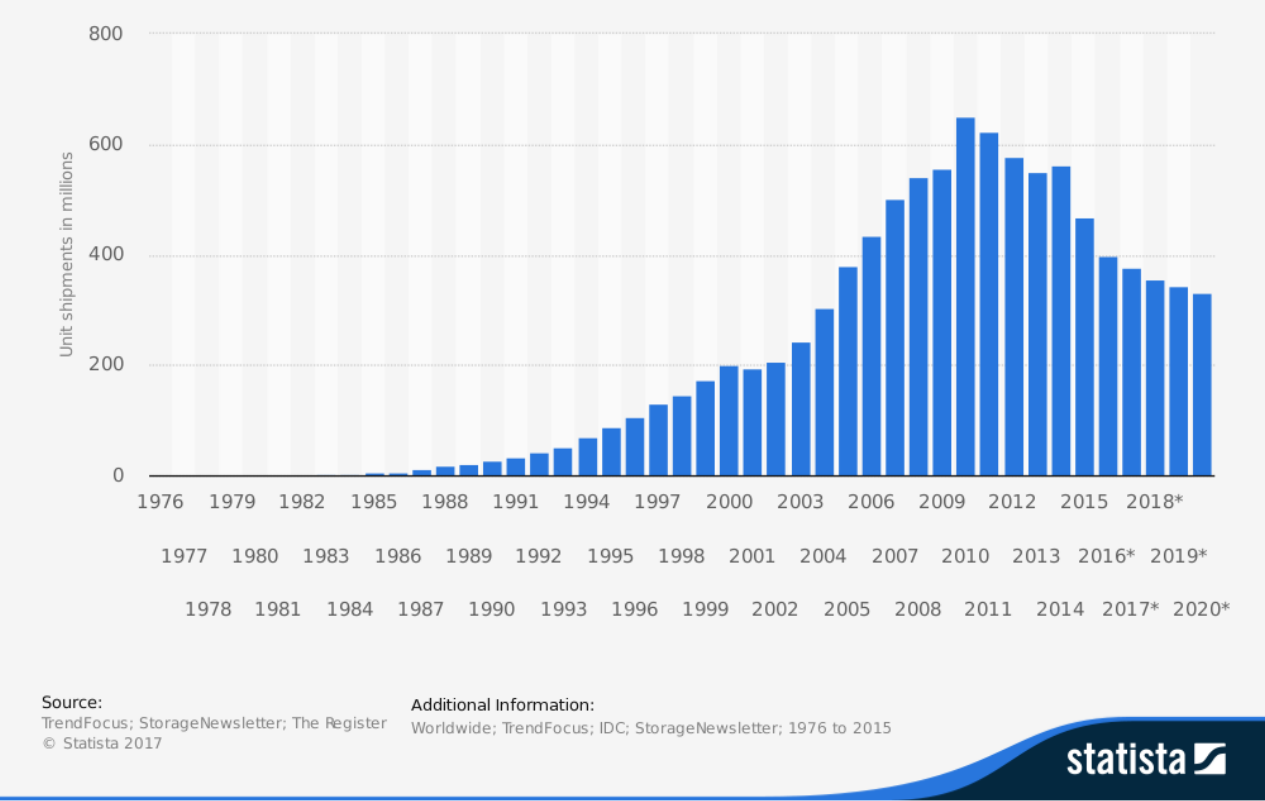
\includegraphics[width=\textwidth]{images/HDDUnitShipments.png}
   Evolution of Worldwide Unit Shipments of Hard Disk Drives (HDD) from 1976 to 2020 (Mi).
\end{center}
\end{frame}



\begin{frame}{Spinning Disk Technology}{}
{\Large Technology Evolution}
\bigskip
\begin{itemize}
\item Shingled Magnetic Recording (SMR) disks: 2013
\item Helium-filled disks (more platters): 2013
\item Heat-Assisted Magnetic Recording (HAMR) disks: $\approx$2018
      % The next major step in technology advancement would have been Heat Assisted Magnetic Recording
      % (HAMR), but there are still reliability and yield problems and thus the first drives will only appear in
      % the market in 2018 the earliest.
      % Complex technology, laser + new media, reliability + cost are issues
   % New technologies are more like tape in the way that they behave (append-only, with periodic repacks)
\end{itemize}
\bigskip
{\Large Capacity/Pricing Evolution}
\bigskip
\begin{itemize}
   \item Next 3--12 months: 14--16 Tb
   \item By 2020: 20 Tb
   \item By $\approx$2025: 100 Tb with HAMR/HDMR % Heated Dot Magnetic Recording
   \item ``Nearline'' disks cost $\approx$35--40 CHF/Tb {\color{red}($-$14\%/year)}
   \item Very shaky price evolution
\end{itemize}
\end{frame}



\begin{frame}{Spinning Disk Technology}{Source: \citealias{astc_roadmap}{ASTC (2016)}}
\begin{textblock}{90.0}[0.5,1](0,67) % {block width} (coords)
\includegraphics<1>[width=\textwidth]{images/ATSCRoadmap0.png}
\includegraphics<2>[width=\textwidth]{images/ATSCRoadmap1.png}
\end{textblock}
\end{frame}



\begin{frame}{SSD Market}
\begin{itemize}
   \item Shipped capacity in 2016: $\approx$45 Eb
   \item SSD shipped capacity is $\approx$7.5\% of HDD shipped capacity. Expected to grow to 20\% by 2021.
   \item Large investments required for SSD manufacturing (\$200--300 Bn)
   \item SSD price/Tb expected to be $\mathcal{O}$(10)$\times$ HDD price/Tb price for the forseeable future
\end{itemize}
\end{frame}



\section{Alternatives to Tape}
\subsection{Alternatives to Tape}

\begin{frame}{Disk Servers for Archival}{}
{\Large Current CERN EOS disk servers}
\bigskip
\begin{itemize}
   \item One CPU node and 2$\times$24 enterprise-class disks
   \item JBOD with 2 replicas
   \item Disk cost is 75\%
   \item TCO is $\approx$3$\times$ tape CHF/Tb
\end{itemize}
\bigskip
{\Large Investigation into ``Monster'' disk servers to optimise disk-to-infrastructure cost ratio}
% to close gap with tape
\bigskip
\begin{itemize}
   \item Use commodity disks to optimise CHF/Tb
   \item \textit{\`{a} la} BackBlaze (30--40\% cheaper)~\citealias{backblaze}{[{\color{cern@ltblue}BackBlaze (2015)}]}
\end{itemize}
\end{frame}



\begin{frame}{Massive Array of Inexpensive Disks (MAID)}{Source: \citealias{monster_nodes}{CERN (2016)}}
\begin{textblock}{52.4}[0.95,1](0,68.8) % {block width} (coords)
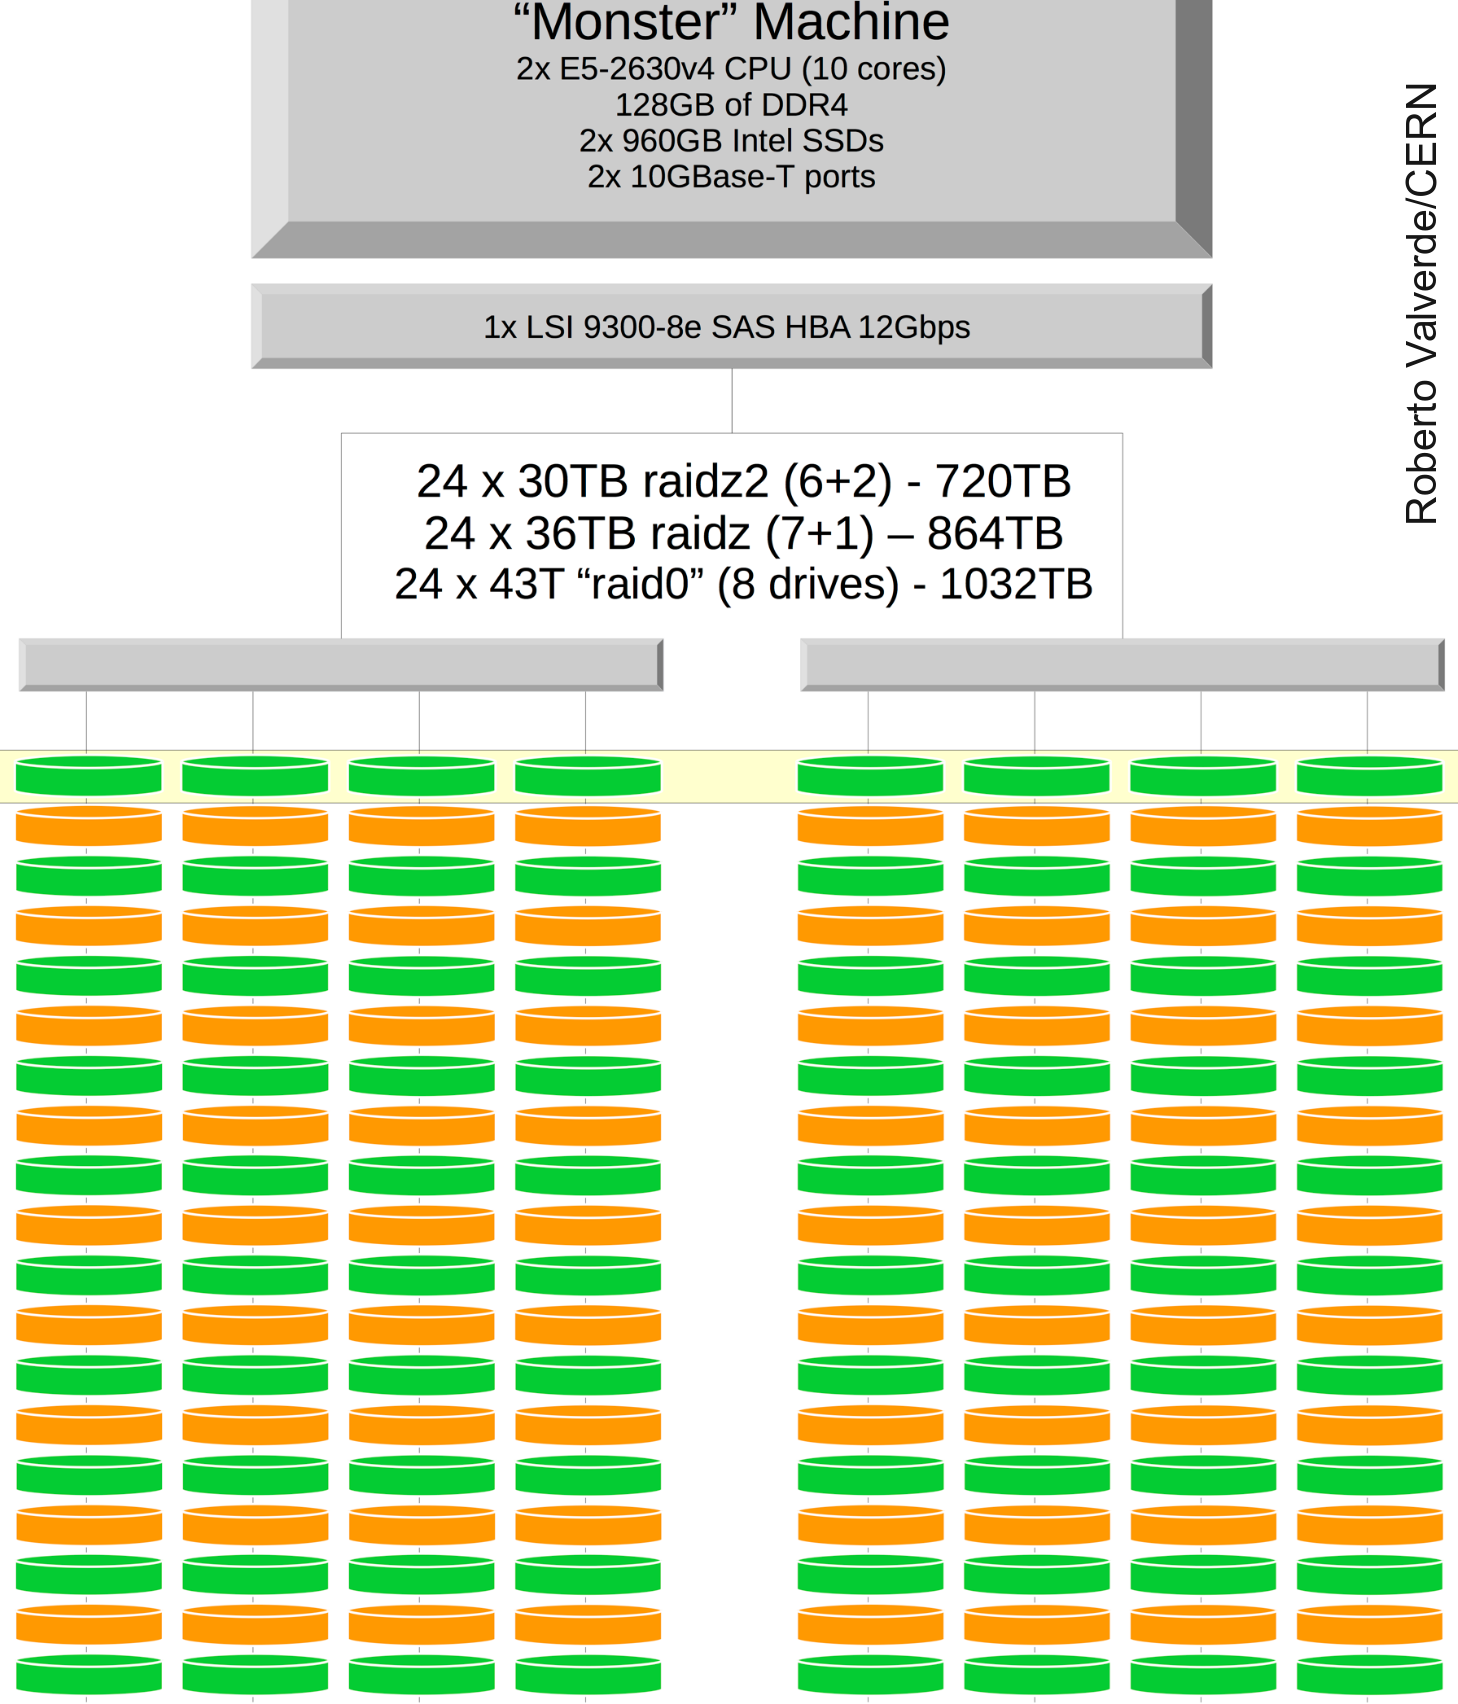
\includegraphics[width=\textwidth]{images/MonsterMachine.png}
\end{textblock}
\only<1>{
\begin{textblock}{45}[1,0](47,10) % {block width} (coords)
\begin{itemize}
   \item Testing 192 disks on one server (2 trays with 8$\times$24 HDDs each)
   \item Up to 1.1 Pb raw (using 6 Tb disks)
   \item Evaluate different file system and redundancy layouts (RAID, erasure coding,\ldots) $\rightarrow$\\[0.5ex]
      \textit{f}(capacity, reliability, performance)
\end{itemize}
\end{textblock}
}\only<2>{
\begin{textblock}{45}[1,0](47,10) % {block width} (coords)
\begin{itemize}
   \item No warranty/certification for our use case
   \item Measure reliability of different models/vendors (integrity, failure rates) using SMART and EOS monitoring
   \item Compensate lower reliability with higher redundancy
   \item Review operating procedures: let disks die rather than replacing
   \item Two servers in production for ALICE (successfully so far)
\end{itemize}
\end{textblock}
}
\end{frame}



% Archival Disk---evolution of Blu-Ray
% Collaboration between Sony and Panasonic
% Max capacity 300 Gb disks (WORM only)
% 140 Mb/s write, 280 Mb/s read
% Reliability (Blu-Ray UBER $10^{-12}$) $\rightarrow$ erasure coding overhead
% Roadmap to 1 Tb but no timeline nor new products
% ``1 Tb by''\ldots (was 2010, then 2012, now 2020\ldots)
% Consumer market for optical disks vanishing
% Behind magnetic storage in capacity, performance, reliability
% Media volumes, pricing? ``Cheaper than HDD''
\begin{frame}{Optical}{}
\begin{textblock}{100.0}[0.5,1](0,70) % {block width} (coords)
\begin{center}
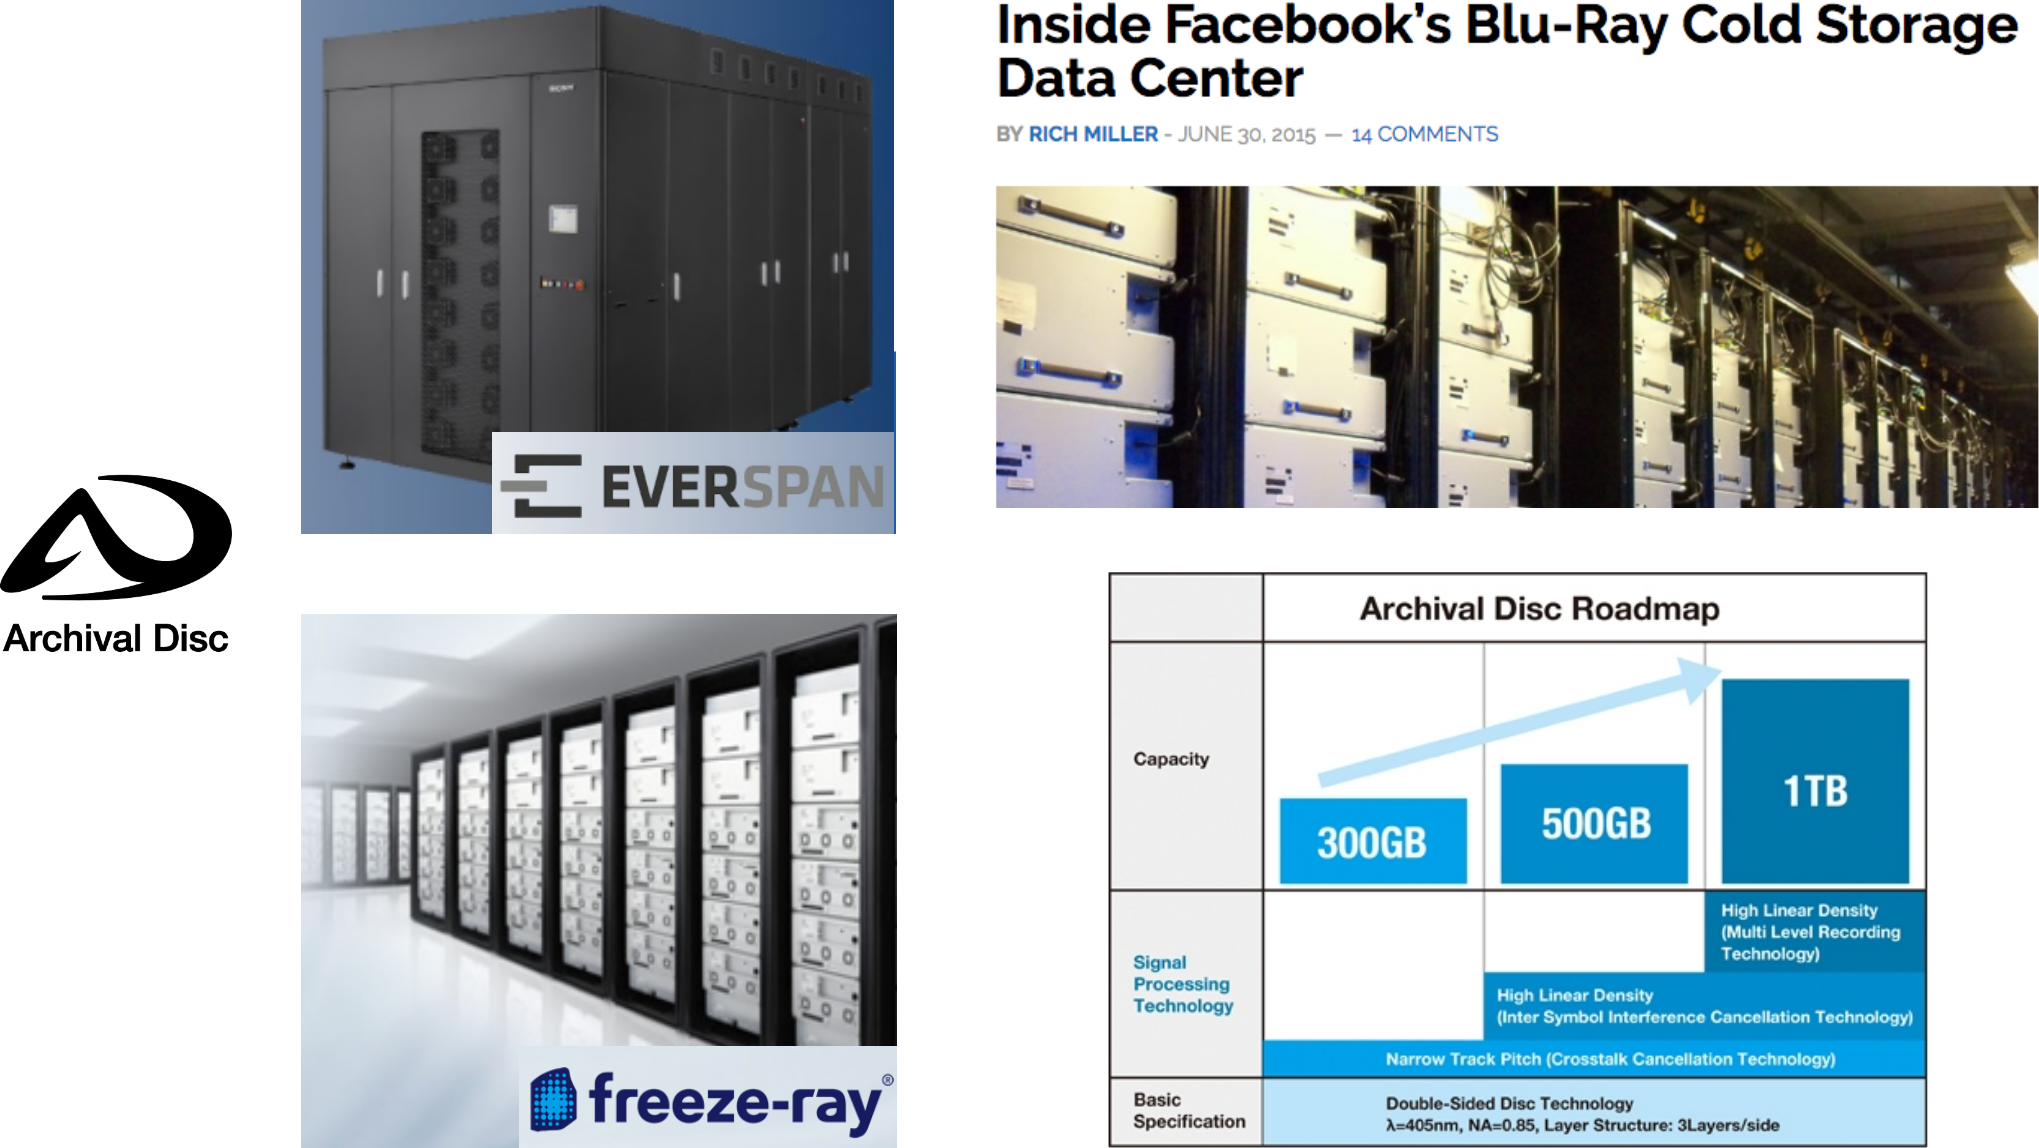
\includegraphics[width=0.95\textwidth]{images/Optical.png}
\end{center}
\end{textblock}
\end{frame}



% Libraries announced by Sony (Everspan) and Panasonic (Freeze-Ray)
% Robots mounting media trays for 4$\times$16 disks (Everspan)/12 disks (Freeze-Ray)
% Up to 14 expansion media racks @ 13 Pb raw (Everspan) $\rightarrow$ $\approx$180 Pb
% Up to 64 drives/library (Everspan)
\begin{frame}{Optical Libraries}{Source: \citealias{optical_library}{Sony}}
\begin{textblock}{100.0}[0.5,1](0,70) % {block width} (coords)
\begin{center}
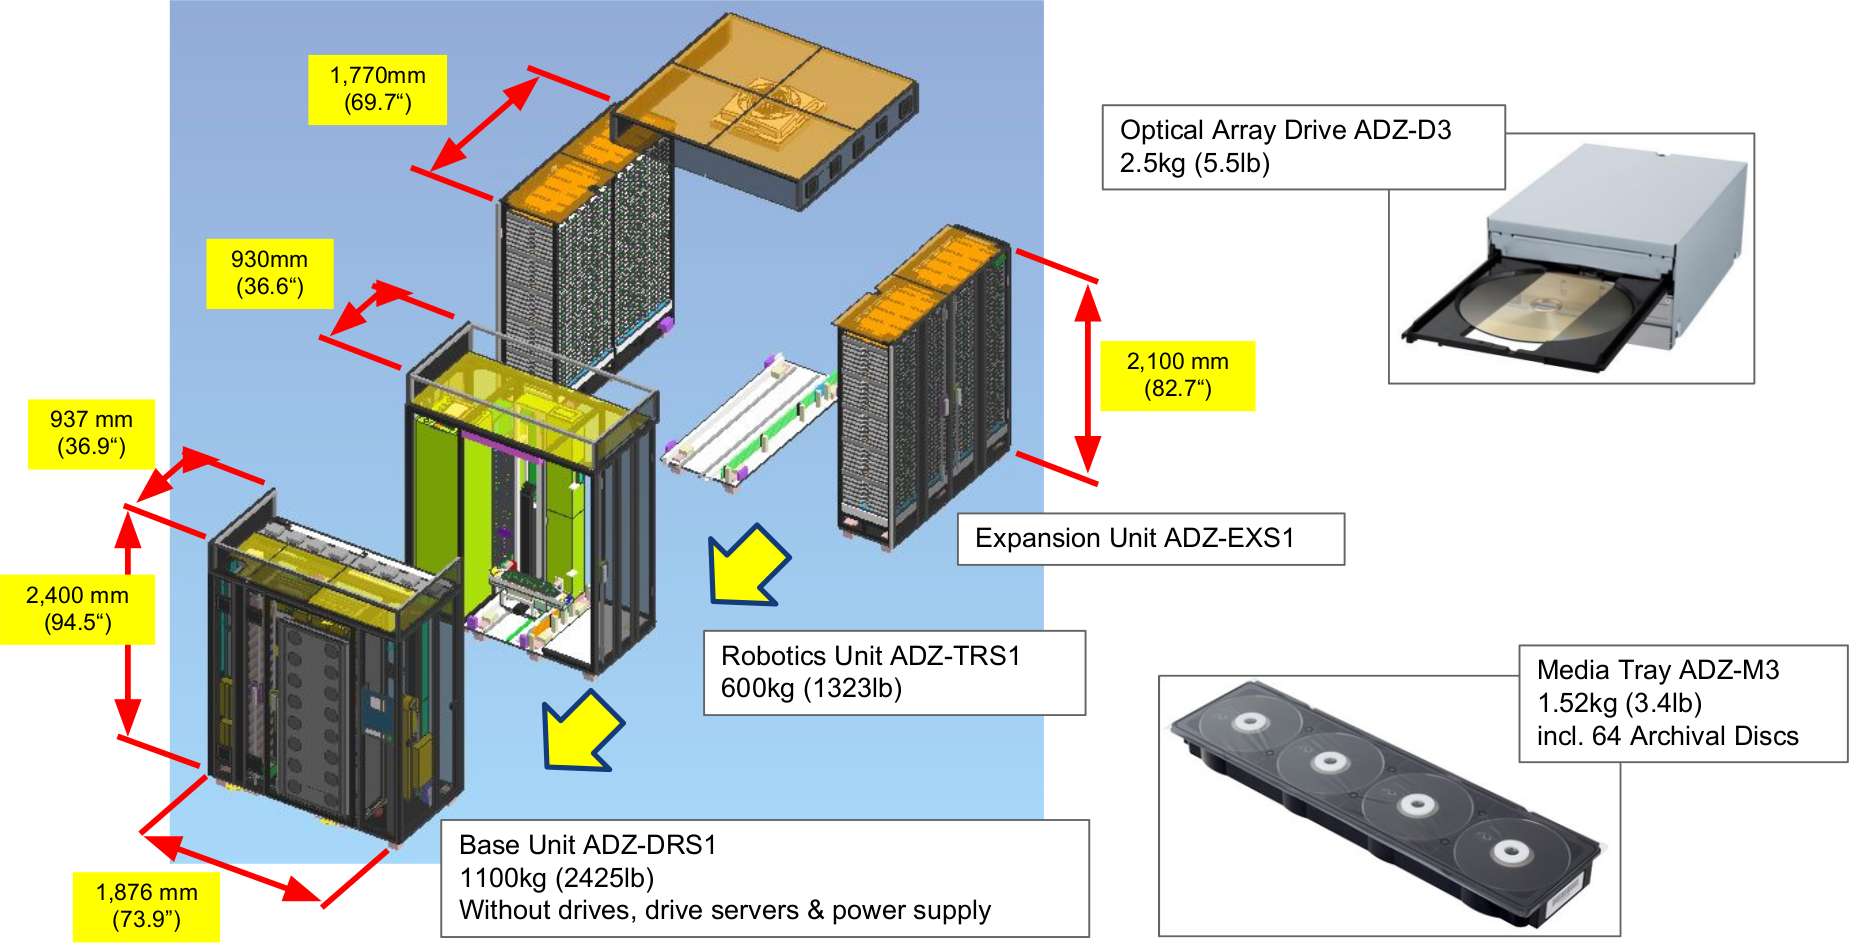
\includegraphics[width=0.95\textwidth]{images/OpticalLibrary.png}
\end{center}
\end{textblock}
\end{frame}



\begin{frame}{Holographic}{Source: \citealias{holographic}{Akonia Holographics (2015)}}
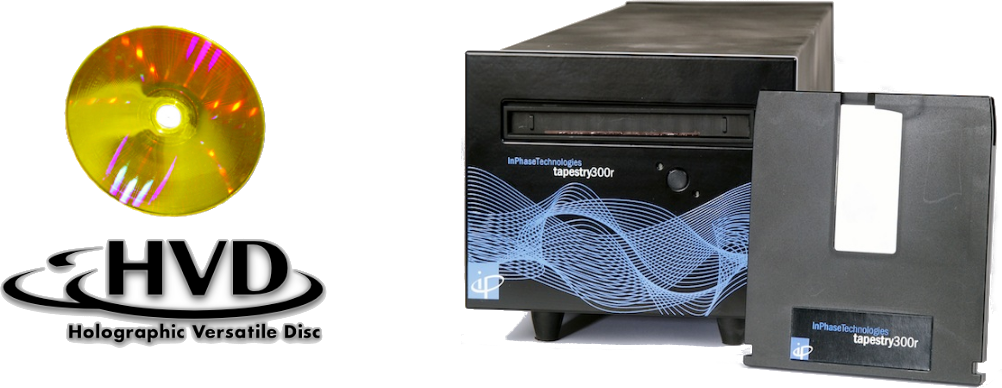
\includegraphics[width=\textwidth]{images/Holographic.png}
\begin{itemize}
   \item Record information across media volume, not just surface
   \item High densities using different recording angles, wavelengths, position on single media location
   \item Potentially, $\mathcal{O}(Gb)/mm^{3}$, fast R/W rates
   %\item 2015 Demo: $2 Tb/in^{2} \rightarrow \approx$770 Gb/in 3
   \item Prototypes, even ECMA standards
   %\item 300 Gb/disk, 20 Mb/s
   %\item Small companies: InPhase (bankrupt in 2011), Akonia Holographics
   %\item Research @ IBM Almaden Labs (until $\approx$2000); GE
   \item No products on the market, nor any signs of upcoming ones
\end{itemize}
\end{frame}



\section{Archival at CERN}
\subsection{Archival at CERN}

\begin{frame}{CERN Tape Archive}{Source: \citealias{hepix2017}{CERN/HEPiX (2017)}}
\begin{textblock}{100.0}[0.5,1](0,70) % {block width} (coords)
\begin{center}
\includegraphics<1>[width=0.9\textwidth]{images/CTA0.png}
\includegraphics<2>[width=0.9\textwidth]{images/CTA1.png}
\end{center}
\end{textblock}
\end{frame}



% We asked for RAO, we got it in Enterprise Drives, but if there are no Oracle drives and we go to
% LTO-8 we may lose it again.
\begin{frame}{Recommended Access Order}{Source: \citealias{cristina}{Cristina Moraru (2017)}}
\begin{textblock}{100.0}[0.5,1](0,67) % {block width} (coords)
\begin{center}
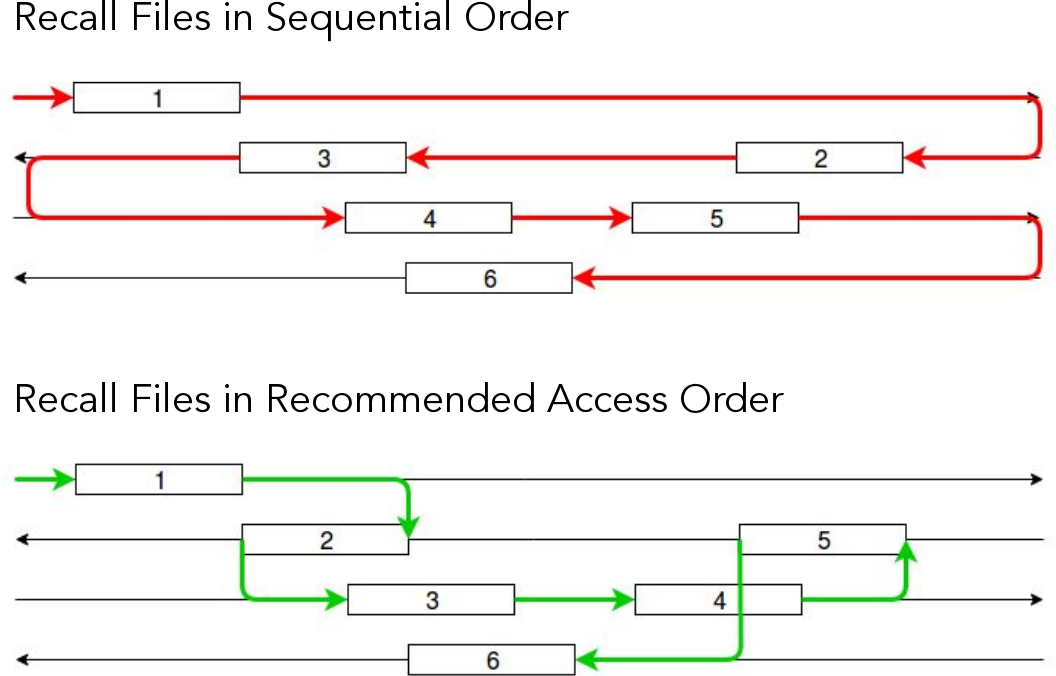
\includegraphics[width=0.8\textwidth]{images/RAO0.png}
\end{center}
\end{textblock}
\end{frame}



\begin{frame}{Recommended Access Order}{Source: \citealias{cristina}{Cristina Moraru (2017)}}
\begin{textblock}{100.0}[0.5,1](0,67) % {block width} (coords)
\begin{center}
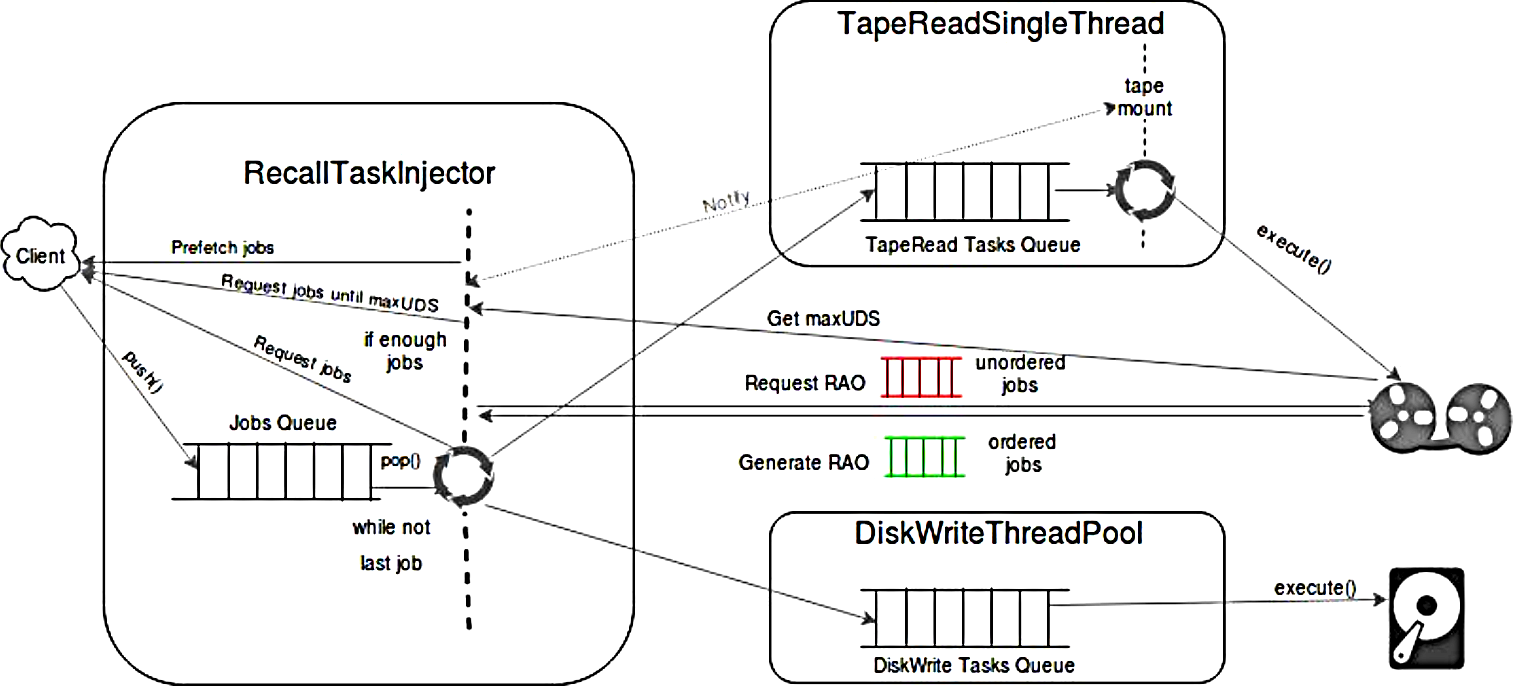
\includegraphics[width=0.9\textwidth]{images/RAO1.png}
\end{center}
\end{textblock}
\end{frame}



\begin{frame}{Recommended Access Order}{Source: \citealias{cristina}{Cristina Moraru (2017)}}
\begin{textblock}{100.0}[0.5,1](0,67) % {block width} (coords)
\begin{center}
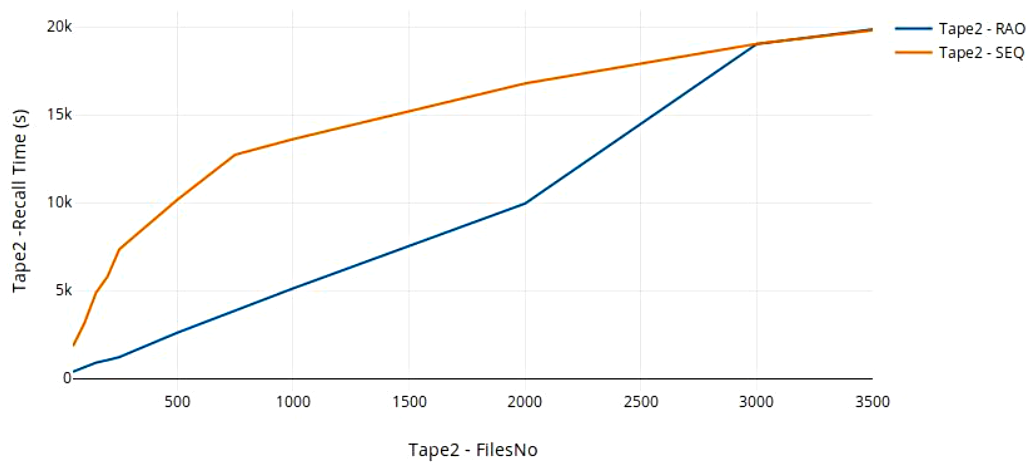
\includegraphics[width=0.9\textwidth]{images/RAO2.png}
\end{center}
\end{textblock}
\end{frame}



\begin{frame}{Summary}{}
\begin{itemize}
   \item Tape is still the most cost-effective archival solution for HEP\\[1ex]
      \textbf{BUT:}\\[1ex]
   \item Concerns about the long-term sustainability of a tape market dominated by a
      single technology provider
\end{itemize}

{\Large Mitigating Market Risks}

\begin{itemize}
   \item Investigate massive commodity disk setup (MAID) for archival
   \item Keep an eye on optical storage
\end{itemize}
\end{frame}



%%
%% Closing page
%%

\section{}

\begin{frame}[allowframebreaks]{References}{}
\bibliography{OutlookForArchivalStorageAtCERN_MichaelDavis}
\bibliographystyle{unsrt}
\end{frame}

{
\setbeamertemplate{headline}{}
\begin{frame}{}{}
\begin{textblock}{140.0}[0.5,1](0,72) % {block width} (coords)

\includegraphics[width=\textwidth]{images/CERN_logo_bg}
\end{textblock}
\end{frame}
}

\end{document}
